%%%%%%%%%%%%%%%%%%%%%%%%%%%%%%%%%%%%%%%%%
% University/School Laboratory Report
% LaTeX Template
% Version 3.1 (25/3/14)
%
% This template has been downloaded from:
% http://www.LaTeXTemplates.com
%
% Original author:
% Linux and Unix Users Group at Virginia Tech Wiki 
% (https://vtluug.org/wiki/Example_LaTeX_chem_lab_report)
%
% License:
% CC BY-NC-SA 3.0 (http://creativecommons.org/licenses/by-nc-sa/3.0/)
%
%%%%%%%%%%%%%%%%%%%%%%%%%%%%%%%%%%%%%%%%%

%----------------------------------------------------------------------------------------
%	PACKAGES AND DOCUMENT CONFIGURATIONS
%----------------------------------------------------------------------------------------

\documentclass{article}

%\usepackage[version=3]{mhchem} % Package for chemical equation typesetting
%\usepackage{siunitx} % Provides the \SI{}{} and \si{} command for typesetting SI units
\usepackage{graphicx} % Required for the inclusion of images
%\usepackage{natbib} % Required to change bibliography style to APA
\usepackage{amsmath} % Required for some math elements 
\usepackage{float}
\usepackage{changepage}



\setlength\parindent{0pt} % Removes all indentation from paragraphs

%\renewcommand{\labelenumi}{\alph{enumi}.} % Make numbering in the enumerate environment by letter rather than number (e.g. section 6)

%\usepackage{times} % Uncomment to use the Times New Roman font

%----------------------------------------------------------------------------------------
%	DOCUMENT INFORMATION
%----------------------------------------------------------------------------------------

\title{Fundaments of HPC \\ Third Assignment \\ Exercise 1: The Mandelbrot Set} % Title

\author{Nicola \textsc{Domenis}} % Author name

\date{\today} % Date for the report

\begin{document}

\maketitle % Insert the title, author and date

\begin{center}
\begin{tabular}{l r}

\end{tabular}
\end{center}

% If you wish to include an abstract, uncomment the lines below
% \begin{abstract}
% Abstract text
% \end{abstract}

%----------------------------------------------------------------------------------------
%	SECTION 1
%----------------------------------------------------------------------------------------

\section{Introduction}

We present the second assignment in the course of FHPC. We will discuss about:


% If you have more than one objective, uncomment the below:
\begin{description}
\item[Main Exercise] \hfill \\
Creation of an openmp code capable of rendering images of the Mandelbrot set;
\item[Secondary Exercise] \hfill \\
Testing the strong and weak scalability of the program;

\end{description} 
 
%----------------------------------------------------------------------------------------
%	SECTION 2
%----------------------------------------------------------------------------------------

\section{Main exercise: visualizing Mandelbrot sets}

We started by implementing the serial program as "serial\_mandelbrot.c". We followed the instructions on the assignment.
We use the input data to create a matrix that will contain the values that count the steps of the series to reach non-convergence, given by the condition $\left|z\right|>2$.
There are three nested for cycles. Two for cycles are used to scan the matrix and one verifies if the point to which the cells refers to belongs or not to the mandelbrot set.
Then we recognized that to parallelize this problem it was necessary to act on the main for cycle. We added an OMP for command to deal with the parallelization.
Then we tested the program with various parameters. Notably we risk of exhausting the memory of the computer if we make a too big matrix. Having a large number of iterations is also a source of computational effort from the machine. Finally, the two points of input might be problematic to explore the Mandelbrot set, since it is easy to miscalculate the position and end up into a zone that fully belongs to the Mandelbrot set, thus being uninteresting. 
Interesting results came up by substituting the series formula $z_{n+1} = z^{2}_n + c$ with other formulas. We report some interesting images:




\begin{figure}[H] % [h] forces the figure to be output where it is defined in the code (it suppresses floating)
	\centering
	\includegraphics[width=0.5\columnwidth]{images/parallel_mandelbrot_image_peculiar_1.jpg} % Example image
	\caption{Representation of the Mandelbrot set}
\end{figure}

\begin{figure}[H] % [h] forces the figure to be output where it is defined in the code (it suppresses floating)
	\centering
	
\includegraphics[width=0.5\columnwidth]{images/mandelbrot_image_peculiar_1} % Example image
	\caption{Particular of the Mandelbrot set}
\end{figure}

\begin{figure}[H] % [h] forces the figure to be output where it is defined in the code (it suppresses floating)
	\centering
	
\includegraphics[width=0.5\columnwidth]{images/mandelbrot_image_peculiar_17} % Example image
	\caption{Deep particular of the Mandelbrot set}
\end{figure}




\begin{figure}[H] % [h] forces the figure to be output where it is defined in the code (it suppresses floating)
	\centering
	
\includegraphics[width=0.5\columnwidth]{images/custom_mandelbrot_image_cubic_peculiar_9} % Example image
	\caption{Mandelbrot set using $z_{n+1} = z^{3}_n + c$}
\end{figure}

\begin{figure}[H] % [h] forces the figure to be output where it is defined in the code (it suppresses floating)
	\centering
	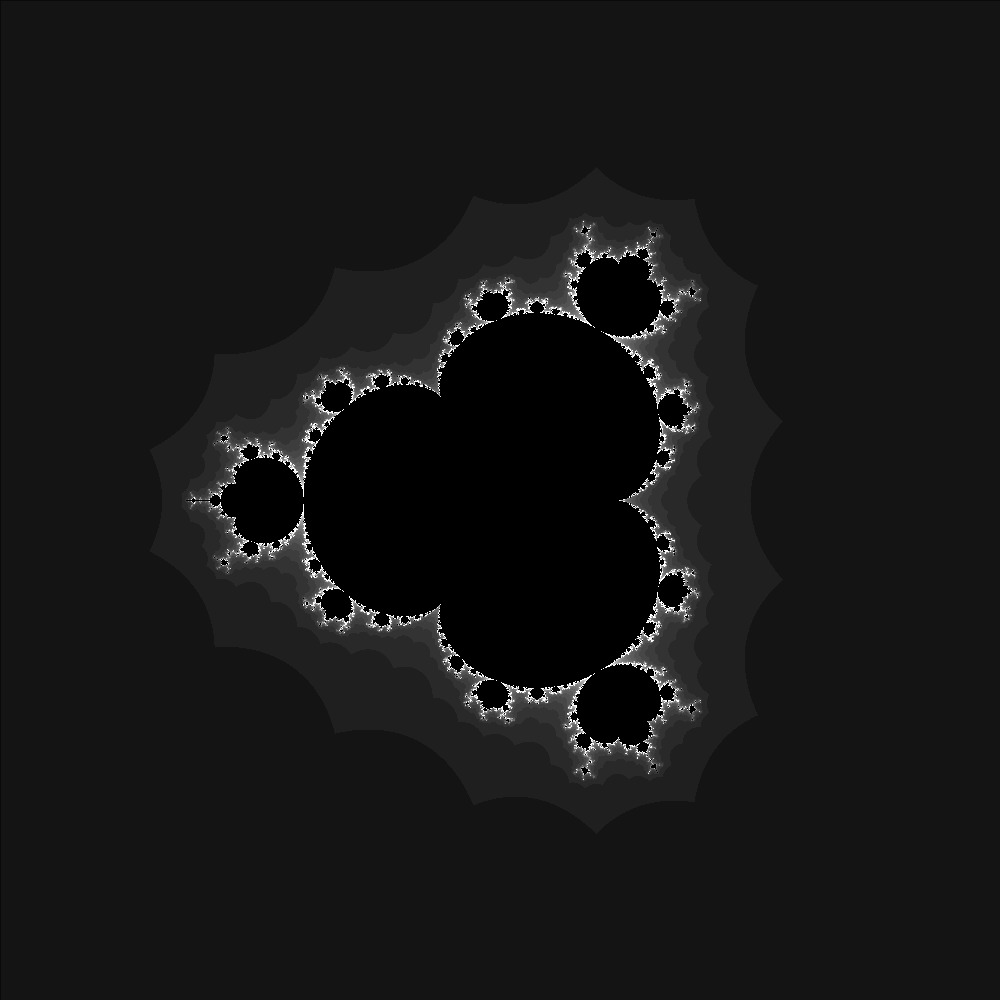
\includegraphics[width=0.5\columnwidth]{images/custom_mandelbrot_image_cubic_tetrahedric_10} % Example image
	\caption{Mandelbrot set using $z_{n+1} = z^{4}_n + c$}
\end{figure}

\begin{figure}[H] % [h] forces the figure to be output where it is defined in the code (it suppresses floating)
	\centering
	
\includegraphics[width=0.5\columnwidth]{images/custom_mandelbrot_image_pentapower_peculiar_10} % Example image
	\caption{Mandelbrot set using $z_{n+1} = z^{5}_n + c$}
\end{figure}

\begin{figure}[H] % [h] forces the figure to be output where it is defined in the code (it suppresses floating)
	\centering
	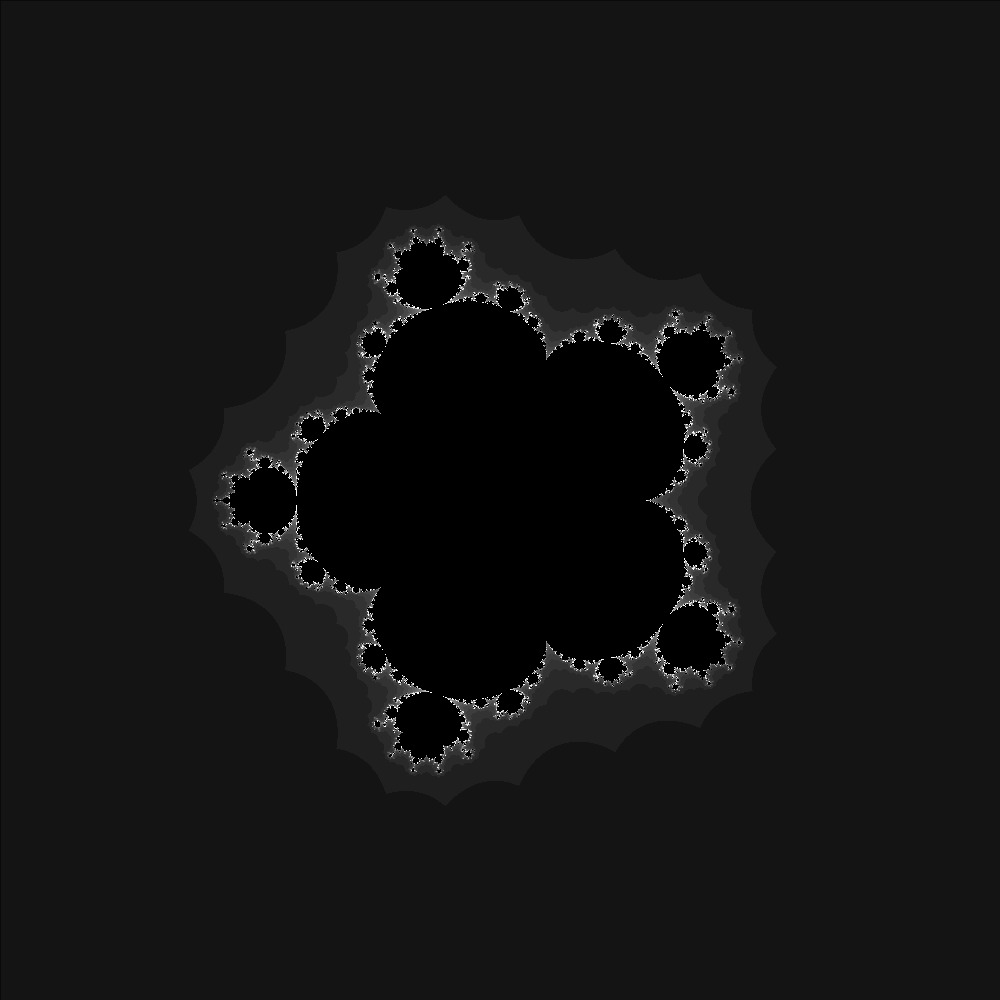
\includegraphics[width=0.5\columnwidth]{images/custom_mandelbrot_image_esapower_peculiar_11} % Example image
	\caption{Mandelbrot set using $z_{n+1} = z^{6}_n + c$}
\end{figure}

\section{Strong and Weak Scalability Test}
We report the graphs of the elapsed time during the strong and weak scalability tests:


\begin{figure}[H] % [h] forces the figure to be output where it is defined in the code (it suppresses floating)
	\centering
	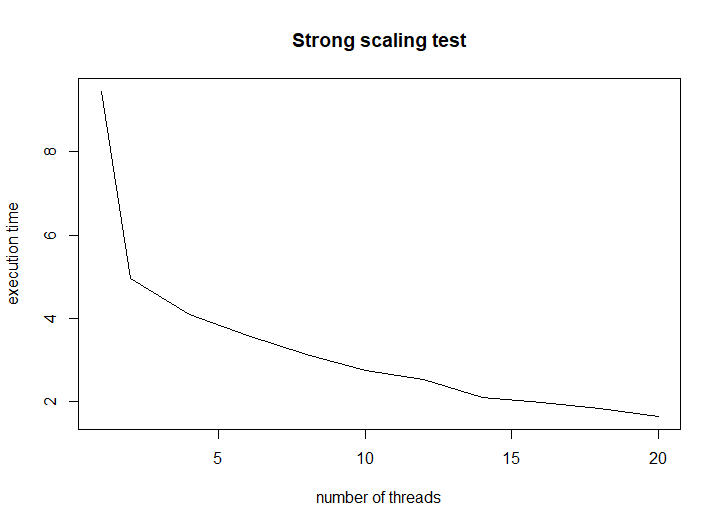
\includegraphics[width=0.8\columnwidth]{graphs/strong_scaling_test_mandelbrot} % Example image
	\caption{Strong scaling test for $N=10^4$ }
\end{figure}
\begin{figure}[H] % [h] forces the figure to be output where it is defined in the code (it suppresses floating)
	\centering
	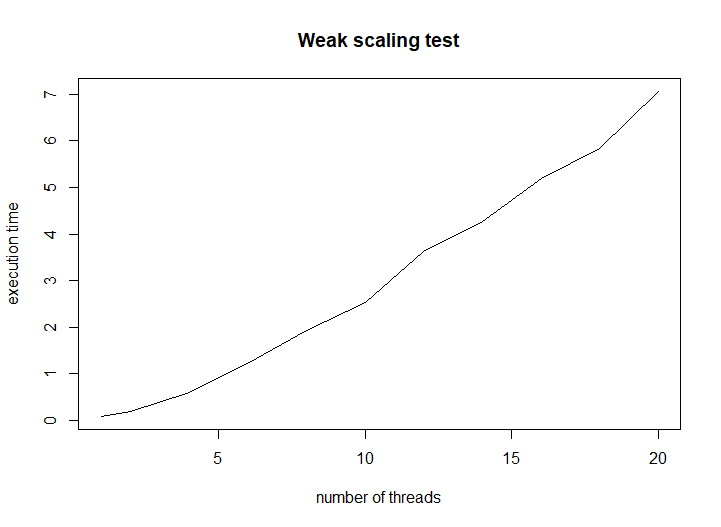
\includegraphics[width=0.8\columnwidth]{graphs/weak_scaling_test_mandelbrot} % Example image
	\caption{Weak scaling test for $N=10^3$multiplied by the number of threads}
\end{figure}
We see that the code scales well in the strong scaling case, while it doesn't have a constant execution time while we execute the weak scaling test. The reason for this might be that the workscale isn't distributed very well among the threads. 

\section{Solving the workload imbalance}
We can add a schedule clause in the pragma command to evenly distribute the workload among the task. If we execute "parallel\_mandelbrot" and then "parallel_mandelbrot_scheduling" we can see that in the second case the execution time for all threads is balanced.
We 


%----------------------------------------------------------------------------------------
%	SECTION 5
%----------------------------------------------------------------------------------------



%----------------------------------------------------------------------------------------
%	SECTION 6
%----------------------------------------------------------------------------------------


%----------------------------------------------------------------------------------------
%	BIBLIOGRAPHY
%----------------------------------------------------------------------------------------
%---------------------------------------------------------------------------------------


\end{document}